\documentclass[11pt,a4paper,oneside]{report}
\usepackage[a4paper,margin=2.3cm]{geometry}
\usepackage{fontspec}
\setmainfont{Liberation Serif}
\setsansfont{Liberation Sans}
\usepackage{polyglossia}
\setdefaultlanguage{vietnamese}
\usepackage{amsmath,amssymb}
\usepackage{booktabs,tabularx,array,longtable}
\usepackage{graphicx}
\graphicspath{{img/}{deepfig/}{../06_code/results/data_story/}{../06_code/results/dataset_deep_analysis/figures/}}
\usepackage{xcolor}
\usepackage{enumitem}
\usepackage[ruled,vlined,linesnumbered]{algorithm2e}
\usepackage{tikz}
\usetikzlibrary{arrows.meta,positioning,fit}
\usepackage{caption}
\usepackage{pgfplots}
\pgfplotsset{compat=1.18}
\usepackage[most]{tcolorbox}
\usepackage{titlesec}
\titleformat{\chapter}[hang]{\normalfont\LARGE\bfseries\color{teal}}{\thechapter}{0.6em}{}
\titlespacing*{\chapter}{0pt}{-10pt}{14pt}
\usepackage{hyperref}
\definecolor{teal}{HTML}{0F4C4F}
\definecolor{tealmid}{HTML}{2E7D7A}
\definecolor{tealpale}{HTML}{E6F0EF}
\definecolor{amber}{HTML}{E89B2D}
\definecolor{amberpale}{HTML}{FCF1DF}
\definecolor{coral}{HTML}{C8553D}
\hypersetup{colorlinks=true,linkcolor=teal,urlcolor=tealmid,citecolor=tealmid,pdftitle={Luận văn GRAPES-GFN-Rec (bản sống)}}
\newcolumntype{Y}{>{\raggedright\arraybackslash}X}
\setlist{itemsep=2pt,topsep=4pt}
\captionsetup{font=small,labelfont=bf}
\SetAlgorithmName{Thuật toán}{thuật toán}{Danh sách thuật toán}

\newcommand{\pending}[2]{\begin{tcolorbox}[colback=amberpale,colframe=amber,boxrule=0.8pt,arc=2pt,left=6pt,right=6pt,top=4pt,bottom=4pt,fontupper=\small]\textbf{\color{coral}ĐANG CHỜ} · \textbf{#1}\\ #2\end{tcolorbox}}
\newcommand{\rstar}{\ensuremath{\bigstar}}
\newcommand{\docversion}{0.4}
\newcommand{\docdate}{16/09/2026}
\title{\textbf{Học cách lấy mẫu đồ thị cho hệ gợi ý quy mô lớn dùng GNN}\\[6pt]\Large GRAPES-GFN-Rec trên Amazon Reviews'23 Baby\_Products\\[10pt]\normalsize Luận văn --- bản sống \docversion}
\author{Ty Van Xuan}
\date{Cập nhật \docdate}
\begin{document}
\maketitle
\begin{abstract}
\noindent Luận văn chuyển GRAPES \cite{grapes} --- phương pháp lấy mẫu đồ thị trong đó một GNN phụ học chọn node cho từng layer bằng GFlowNet --- sang hệ gợi ý. Phương pháp đề xuất, GRAPES-GFN-Rec, học chọn node ngữ cảnh cho Sampled LightGCN \cite{lightgcn} với phần thưởng từ BPR ranking loss \cite{bpr} và Trajectory Balance \cite{tb}, rồi được so sánh với lấy mẫu đều, lấy mẫu theo bậc, biến thể REINFORCE, Full LightGCN, MostPop và BPR-MF dưới cùng protocol. Dữ liệu là Amazon Reviews'23 Baby\_Products \cite{amazon23}: graph huấn luyện 3.868.654 cạnh, 2.318.308 user, 162.125 sản phẩm, rất thưa (71,76\% user một tương tác) và lệch long-tail (Gini 0,858). Đây là bản sống: chương dữ liệu, trả lời góp ý và phương pháp đã có; kết quả thực nghiệm được điền theo từng gate.
\end{abstract}
\tableofcontents
%=====================================================================
\chapter*{Trạng thái tài liệu và nhật ký cập nhật}
\addcontentsline{toc}{chapter}{Trạng thái tài liệu và nhật ký cập nhật}
Đây là \textbf{bản sống} của luận văn: mỗi gate hoàn thành sẽ điền thêm vào đúng chương, không viết lại từ đầu. Phần đóng khung ``ĐANG CHỜ'' chưa có số liệu và ghi rõ nguồn sẽ điền.

\begin{center}\small
\begin{tabularx}{\linewidth}{p{3.2cm}Yp{2.6cm}p{2.6cm}}
\toprule
Chương & Nội dung & Trạng thái & Điền tiếp khi \\
\midrule
1 Mở đầu & Bùng nổ lân cận, sampling vs distributed, GRAPES, câu hỏi nghiên cứu & Có & -- \\
2 Dữ liệu & Chất lượng, rating, histogram, long-tail, cold-start, thời gian, bất thường, đồng mua, lân cận, metadata, dev split & Có & -- \\
3 Góp ý giảng viên & Trả lời từng câu hỏi ngày 3/9 & Có; số theo mô hình chờ & R5, R6 \\
4 Phương pháp & GRAPES-GFN-Rec & Có & R2 hoàn tất \\
5 Thiết kế thực nghiệm & So sánh, chỉ số, tiêu chí & Có & R4 \\
6 Kết quả & Development, holdout, hành vi sampler, budget & Đang chờ & R3, R5, R6 \\
7 Kết luận & Tổng kết, hạn chế, hướng phát triển & Đang chờ & R7 \\
\bottomrule
\end{tabularx}
\end{center}

\noindent\textbf{Nhật ký.}
\begin{itemize}
\item \textbf{0.4 (16/09/2026)} Điền kết quả notebook 11: rating theo độ phổ biến, bất thường, hành vi thời gian và độ trôi, bùng nổ lân cận đo thực tế, đồng mua và bằng chứng collaborative cho target, metadata, development split (R1 xong). Thêm DL-003.
\item \textbf{0.3 (16/09/2026)} Chuyển sang bản sống; mở rộng chương dữ liệu; thêm chương trả lời góp ý 3/9; kế hoạch nén về hạn nộp 30/11/2026.
\item \textbf{0.2 (16/09/2026)} Đề xuất GRAPES-GFN-Rec; lõi mã R2 với 28 oracle test.
\item \textbf{0.1 (16/09/2026)} Rà soát scope (DL-001): pilot M0--M2 chuyển sang phụ lục.
\end{itemize}

%=====================================================================
\chapter{Mở đầu}

\section{GNN cho hệ gợi ý và bùng nổ lân cận}
Trong collaborative filtering dựa trên đồ thị, user và sản phẩm là node, mỗi tương tác là một cạnh. LightGCN \cite{lightgcn} học embedding bằng cách lan truyền và lấy trung bình embedding của hàng xóm qua $L$ bước, không có ma trận biến đổi hay hàm phi tuyến. Để tính embedding của một user ở độ sâu $L$, model cần toàn bộ vùng lân cận $L$ bước.

Kích thước vùng lân cận tăng theo tích các bậc gặp trên đường đi. Trên graph Baby\_Products, một user trung bình có 1,67 sản phẩm; nhưng đi theo một cạnh ngẫu nhiên, sản phẩm gặp phải có bậc kỳ vọng
\[
  \mathbb{E}_{\text{cạnh}}[\deg(i)] = \frac{\sum_i \deg(i)^2}{\sum_i \deg(i)} \approx 1.009 \text{ user},
\]
lớn hơn rất nhiều so với bậc trung bình 23,9, vì cạnh dồn vào sản phẩm phổ biến. Sản phẩm lớn nhất có 21.348 user. Chỉ sau hai bước, một user có thể kéo theo hàng nghìn user khác; một batch nhiều triplet hợp các vùng này lại. Đây là \emph{bùng nổ lân cận} mà GraphSAGE \cite{graphsage}, FastGCN \cite{fastgcn}, LADIES \cite{ladies}, PinSage \cite{pinsage} tìm cách kiểm soát.

Đo trực tiếp trên graph train, không lấy mẫu (Hình~\ref{fig:explosion}): một batch 1.024 triplet chạm 23,6\% trong 2,48 triệu node sau 1 bước, 44,7\% sau 2 bước và 93,2\% sau 3 bước; batch 4.096 triplet chạm 46,3\%, 65,9\% và 95,1\%; batch 65.536 triplet (cỡ batch của pilot) chạm 86,6\% ngay bước đầu. Với một user ngẫu nhiên, trung vị là 524 user sau 2 bước (p99: 21.348) và 974 sản phẩm sau 3 bước (p99: 12.979); user có $\ge$5 tương tác chạm trung vị 5.483 user và 7.917 sản phẩm.

\begin{figure}[h]
\centering
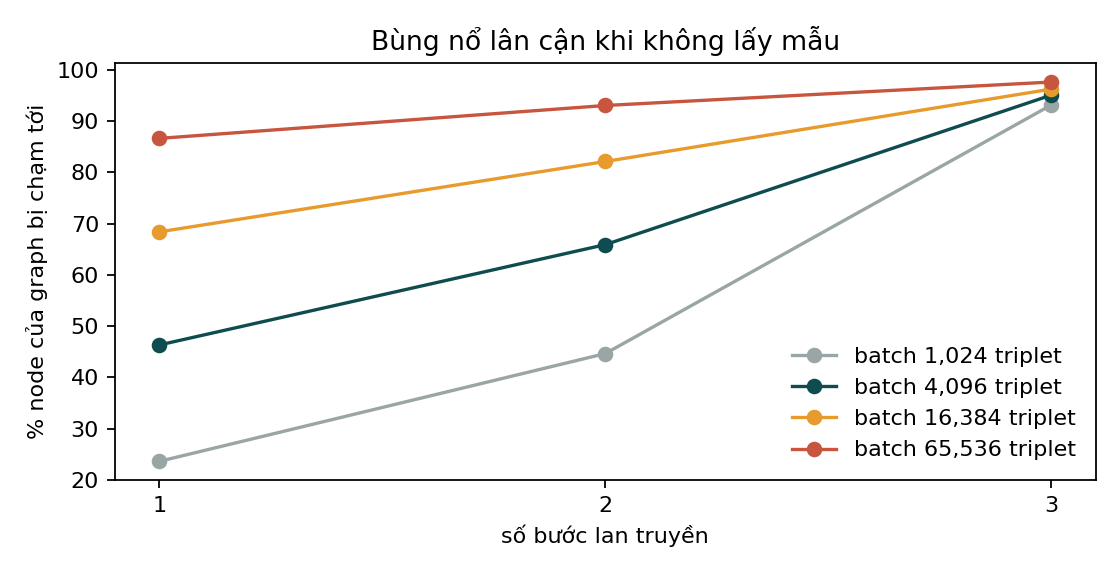
\includegraphics[width=0.72\linewidth]{D4_neighbourhood_explosion.png}
\caption{Tỷ lệ node bị chạm theo số bước lan truyền, không lấy mẫu (3 lần lặp mỗi cỡ batch).}\label{fig:explosion}
\end{figure}

Hệ quả: với batch 65.536 triplet, lấy mẫu gần như không thay đổi context vì graph đã bị phủ gần hết; so sánh sampler có ý nghĩa phải dùng batch nhỏ hơn nhiều (R-1).

\section{Sampling hay distributed?}\label{sec:dist}
Có năm hướng chính để huấn luyện GNN trên graph lớn (Bảng~\ref{tab:dist}).

\begin{table}[h]
\centering\small
\caption{Các hướng mở rộng huấn luyện GNN.}\label{tab:dist}
\begin{tabularx}{\linewidth}{p{2.4cm}YYp{2.1cm}}
\toprule
Hướng & Cách làm & Hạn chế với bài toán này & Vai trò \\
\midrule
Full-graph, 1 GPU & Lan truyền trên toàn graph & Bộ nhớ và thời gian tăng theo số cạnh $\times$ số layer & Tham chiếu \\
Distributed training & Chia batch/model cho nhiều GPU, nhiều máy (PinSage \cite{pinsage}) & Cần cụm máy, chi phí giao tiếp; không giảm lượng tính mỗi batch & Ngoài phạm vi \\
Chia đồ thị & Cluster-GCN \cite{clustergcn}: học trên cụm con & Cắt cạnh giữa cụm; graph lệch hub khó chia đều & Không chọn \\
Embedding lịch sử & GAS \cite{gas}: dùng lại embedding cũ của hàng xóm & Lưu embedding 2,48 triệu node mỗi layer; embedding cũ bị lệch & Không chọn \\
\textbf{Sampling} & \textbf{GraphSAGE, FastGCN, LADIES, GRAPES}: giới hạn $k$ node mỗi layer & Mất ngữ cảnh $\rightarrow$ phải chọn node đúng & \textbf{Hướng chính} \\
\bottomrule
\end{tabularx}
\end{table}

Hai hướng bổ sung cho nhau: distributed nhân phần cứng, sampling giảm lượng tính mỗi batch; sampler học được có thể chạy trong từng worker của hệ distributed. Đồ án chọn sampling vì đề tài hướng tới và giới hạn một GPU T4.

\section{Giai đoạn 1: GRAPES}
GRAPES \cite{grapes} dùng hai GNN: $\mathrm{GCN}_C$ giải bài toán chính và $\mathrm{GCN}_S$ chấm điểm hàng xóm để chọn đúng $k$ node mỗi layer bằng Gumbel Top-$k$ \cite{gumbeltopk}; $\mathrm{GCN}_S$ được huấn luyện bằng GFlowNet Trajectory Balance \cite{tb} hoặc REINFORCE với chi phí là loss của $\mathrm{GCN}_C$.

\begin{table}[h]
\centering\small
\caption{Tái hiện GRAPES ở giai đoạn 1 trên Tesla T4 (accuracy).}\label{tab:phase1}
\begin{tabular}{lcccc}
\toprule
Dataset & GRAPES & Random & Thời gian GRAPES & Thời gian Random \\
\midrule
Cora & 0,8710 & 0,8677 & 56,3 s & 30,5 s \\
Citeseer & 0,7857 & 0,7900 & 94,6 s & 56,0 s \\
ogbn-arxiv & 0,6204 & 0,6128 & 11.114 s & 8.133 s \\
\bottomrule
\end{tabular}
\end{table}
Bài học: lợi thế của sampler học được nhỏ và không đều; sampler tốn thêm 37--85\% thời gian, nên chi phí sampler phải nằm trong so sánh. GRAPES chưa được đánh giá trên recommendation.

\section{Rà soát hướng đi}
Nhánh pilot trước đó so sánh ba luật chọn node cố định (M0 đều, M1 theo bậc, M2 frontier-normalized). M2 mượn hình thức hành động của GRAPES nhưng không có policy học được, log-likelihood, phần thưởng, mục tiêu TB/REINFORCE hay bước cập nhật sampler. Decision log DL-001 xác định lại: giai đoạn 2 hiện thực biến thể GRAPES học được; pilot chuyển phụ lục. Một phương pháp chỉ là \emph{biến thể GRAPES} khi thỏa G1--G7: policy có tham số; exact-$k$ Gumbel Top-$k$; $\log q$; tín hiệu loss gợi ý đã detach; $\log Z(V^0)$ học được; TB/REINFORCE; tham số sampler thực sự thay đổi.

\section{Câu hỏi nghiên cứu}
\begin{description}[leftmargin=1.2cm]
\item[RQ1] Giữ cố định recommender, graph, thứ tự triplet, negative, số bước, budget, seed, evaluator và phần cứng, GRAPES-GFN-Rec có trade-off NDCG@20--chi phí tốt hơn lấy mẫu đều và theo bậc không?
\item[RQ2] Trajectory Balance có ổn định, hiệu quả hơn REINFORCE trên tín hiệu BPR không?
\item[RQ3] Sampler học được chọn node nào (bậc, loại, head/body/tail)? Có khuếch đại thiên lệch phổ biến không?
\item[RQ4] Khi budget $k$ chặt hơn, lợi thế (nếu có) thay đổi thế nào?
\end{description}
Kết quả âm là kết quả hợp lệ.

%=====================================================================
\chapter{Dữ liệu và phân tích}\label{ch:data}

\section{Chọn dataset}
Amazon Reviews'23 \cite{amazon23} có nhiều danh mục, số giao dịch lớn và metadata sản phẩm. Ba danh mục được kiểm toán chính xác trên file tải về (Bảng~\ref{tab:portfolio}).

\begin{table}[h]
\centering\small
\caption{So sánh ba danh mục đã kiểm toán (P4, cùng mốc $t_1$, $t_2$).}\label{tab:portfolio}
\begin{tabular}{lrrr}
\toprule
 & All\_Beauty & Baby\_Products & Home\_and\_Kitchen \\
\midrule
Dòng raw & 693.929 & 5.953.891 & 66.623.880 \\
Tương tác P4 & 494.769 & 4.655.843 & chưa kiểm toán \\
User P4 & 455.579 & 2.769.312 & -- \\
Sản phẩm P4 & 91.187 & 194.722 & -- \\
User chỉ 1 tương tác & 94,16\% & 71,64\% & -- \\
Target validation warm & 1.802 (3,98\%) & 81.871 (21,90\%) & -- \\
\bottomrule
\end{tabular}
\end{table}

All\_Beauty quá thưa để đánh giá (94\% user một tương tác, chỉ 1.802 target warm). Home\_and\_Kitchen lớn hơn Baby 11,2 lần, dành cho stress test sau. Baby\_Products đủ lớn để thấy chi phí lấy mẫu, có long-tail rõ và vẫn chạy được ma trận thí nghiệm trên Colab T4. MovieLens 25M, Gowalla, Yelp2018, MIND, KuaiRec phù hợp câu hỏi khác nên chỉ dùng làm bối cảnh.

\section{Biểu diễn dữ liệu}
File gốc có bốn cột: \texttt{user\_id}, \texttt{parent\_asin}, \texttt{rating}, \texttt{timestamp} (ms). Dữ liệu được biểu diễn thành graph hai phía $G=(U\cup I, E)$: node là user hoặc sản phẩm, cạnh là tương tác 4--5\rstar{} kèm thời điểm. Rating không làm trọng số cạnh; không có feature node, nên mỗi node học một embedding ID. Metadata sản phẩm (title, danh mục, giá) chỉ dùng cho đánh giá ngữ nghĩa, không đưa vào huấn luyện.

\section{Chất lượng dữ liệu và nhiễu}\label{sec:noise}
\begin{table}[h]
\centering\small
\caption{Các kiểu nhiễu và quyết định.}\label{tab:noise}
\begin{tabularx}{\linewidth}{p{3.3cm}p{3.2cm}p{2.9cm}Y}
\toprule
Loại & Mức độ & Quyết định & Lý do \\
\midrule
Rating ngoài 1--5 & 1 dòng (0.0) & Loại & Lỗi rõ ràng \\
Trùng cặp, thiếu ID, sai timestamp & 0 & -- & Kiểm tra chính xác toàn file \\
Rating 1--3\rstar{} & 1.298.047 (21,8\%) & Không làm positive & Tín hiệu không thích hoặc không chắc, không phải lỗi \\
User/sản phẩm 1 tương tác & 71,76\% user; 33,35\% sản phẩm & Giữ, không lọc $k$-core & Long-tail thật; lọc sẽ xóa đúng phần sampling phải xử lý \\
Bot, spam, đánh giá dồn dập & 0,10\% tương tác từ user-ngày $\ge$20 & Giữ, chỉ báo cáo & Quá ít; không có quy tắc xóa đăng ký trước (Bảng~\ref{tab:anomaly}) \\
Thiên lệch phổ biến & Top 1\% giữ 44,1\% & Giữ, báo theo nhóm & Làm lệch chỉ số tổng \\
\bottomrule
\end{tabularx}
\end{table}
Nhiễu dạng lỗi rất ít (1/5.953.891 dòng). 32.050 dòng có timestamp trùng với dòng khác; không dòng nào đúng bằng $t_1$ hay $t_2$. Thách thức chính không phải nhiễu mà là thưa và mất cân bằng.

\begin{table}[h]
\centering\small
\caption{Dấu hiệu bất thường trước $t_1$ (chỉ báo cáo, không loại dòng nào).}\label{tab:anomaly}
\begin{tabularx}{\linewidth}{Yp{4.2cm}p{2.2cm}}
\toprule
Dấu hiệu & Số lượng & Tỷ lệ tương tác \\
\midrule
User đánh giá $\ge$5 sản phẩm trong 1 ngày & 36.470 user-ngày (33.367 user) & 4,90\% \\
User đánh giá $\ge$10 sản phẩm trong 1 ngày & 3.335 user-ngày (3.229 user) & 0,87\% \\
User đánh giá $\ge$20 sản phẩm trong 1 ngày & 197 user-ngày (195 user) & 0,10\% \\
User đánh giá $\ge$50 sản phẩm trong 1 ngày & 0 (tối đa 48) & 0\% \\
Cùng user, cùng timestamp & 66 nhóm, 135 dòng & $\approx$0\% \\
Sản phẩm tăng đột biến ($\ge$50/ngày, $\ge$10$\times$ trung vị) & 32 sản phẩm-ngày, 10 sản phẩm & 3.349 dòng \\
User $\ge$10 rating cùng một mức & 2.610 / 31.882 user & -- \\
\bottomrule
\end{tabularx}
\end{table}
Tín hiệu bất thường chiếm dưới 1\% tương tác; đánh giá theo đợt 5--10 sản phẩm/ngày là hành vi mua sắm bình thường. Đồ án giữ nguyên và ghi nhận như một hạn chế.

\section{Rating và chọn tương tác positive}
\begin{figure}[h]
\centering
\begin{tikzpicture}
\begin{axis}[ybar=0pt, width=0.95\linewidth, height=4.6cm, bar width=12pt, xbar, y dir=reverse,
  ytick={1,2,3,4,5}, yticklabels={1\rstar{},2\rstar{},3\rstar{},4\rstar{},5\rstar{}}, xmin=0, xmax=4.6,
  xlabel={triệu rating}, nodes near coords, nodes near coords style={font=\scriptsize, /pgf/number format/.cd, use comma, fixed, precision=2},
  every axis plot/.append style={fill=tealmid, draw=none}, tick label style={font=\small}, axis lines*=left]
\addplot coordinates {(0.555,1) (0.310,2) (0.433,3) (0.682,4) (3.974,5)};
\end{axis}
\end{tikzpicture}
\caption{Phân bố rating Baby\_Products. Rating trung bình 4,21.}\label{fig:rating}
\end{figure}

Phân bố hình chữ J: 66,7\% là 5\rstar{}, 21,8\% là 1--3\rstar{}, trung bình 4,21, nên 4\rstar{} đã thấp hơn trung bình. Bảng~\ref{tab:policy} so sánh ba cách chọn positive.

\begin{table}[h]
\centering\small
\caption{Độ nhạy theo chính sách positive.}\label{tab:policy}
\begin{tabular}{lrrr}
\toprule
 & Tất cả rating & \textbf{P4: 4--5\rstar{}} & P5: chỉ 5\rstar{} \\
\midrule
Tương tác & 5.953.890 & \textbf{4.655.843} & 3.973.866 \\
User & 3.386.206 & \textbf{2.769.312} & 2.476.012 \\
Sản phẩm & 217.654 & \textbf{194.722} & 182.226 \\
User 1 tương tác & 70,01\% & \textbf{71,64\%} & 73,18\% \\
Sản phẩm 1 tương tác & 31,65\% & \textbf{33,13\%} & 34,34\% \\
Target validation warm & 24,50\% & \textbf{21,90\%} & 20,34\% \\
User validation chưa thấy & 75,07\% & \textbf{77,43\%} & 78,88\% \\
\bottomrule
\end{tabular}
\end{table}

Coi mọi rating là positive sẽ gộp cả 1--3\rstar{} vào tín hiệu ``thích''; chỉ lấy 5\rstar{} làm mất 14,65\% tương tác và tăng cold-start. P4 là điểm cân bằng và được chọn trước khi có kết quả model.

\begin{table}[h]
\centering\small
\caption{Rating theo độ phổ biến sản phẩm (4.886.112 rating trước $t_1$).}\label{tab:ratingpop}
\begin{tabular}{lrrrrrr}
\toprule
Số rating của sản phẩm & 1 & 2--5 & 6--20 & 21--100 & 101--1000 & $>$1000 \\
\midrule
Rating trung bình & 4,07 & 4,13 & 4,17 & 4,19 & 4,25 & 4,31 \\
Tỷ lệ 5\rstar{} & 61,6\% & 63,2\% & 64,3\% & 65,0\% & 67,5\% & 70,1\% \\
Tỷ lệ $\le$3\rstar{} & 26,0\% & 24,0\% & 22,8\% & 22,5\% & 20,7\% & 18,9\% \\
\bottomrule
\end{tabular}
\end{table}
Sản phẩm phổ biến vừa nhiều tương tác vừa được đánh giá tốt hơn, nên tương tác positive P4 còn dồn về head mạnh hơn tương tác thô. Phía user: rating trung bình tăng từ 4,18 (user 1 rating) lên 4,34 (user $>$20 rating); 44,2\% user có $\ge$2 rating cho mọi sản phẩm cùng một mức; 18,1\% user có $\ge$5 rating chỉ cho 5\rstar{}; độ lệch chuẩn trung vị 0,58. Rating phản ánh thói quen người đánh giá nhiều hơn mức thích tuyệt đối, ủng hộ việc dùng tín hiệu nhị phân 4--5\rstar{}.

\section{Bao nhiêu sản phẩm và histogram theo sản phẩm}
Số sản phẩm phụ thuộc bước lọc: 217.654 trong dữ liệu raw $\rightarrow$ 194.722 còn tương tác 4--5\rstar{} $\rightarrow$ 162.125 có trong graph train (trước $t_1$). Coverage dùng 162.125 làm mẫu số.

\begin{figure}[h]
\centering
\begin{tikzpicture}
\begin{axis}[ybar, width=0.95\linewidth, height=5.2cm, bar width=11pt,
  xtick={1,2,3,4,5,6}, xticklabels={1,2--5,6--20,21--100,101--1000,>1000}, ymin=0, ymax=48,
  ylabel={\%}, xlabel={số user đã tương tác với sản phẩm}, legend style={draw=none, font=\small}, legend pos=north west,
  nodes near coords, nodes near coords style={font=\scriptsize, /pgf/number format/.cd, use comma, fixed, precision=1}, axis lines*=left, enlarge x limits=0.1]
\addplot[fill=gray!40, draw=none] coordinates {(1,33.35) (2,32.79) (3,19.87) (4,10.13) (5,3.55) (6,0.31)};
\addplot[fill=teal, draw=none] coordinates {(1,1.40) (2,4.12) (3,8.84) (4,18.65) (5,40.64) (6,26.35)};
\legend{\% sản phẩm, \% tương tác}
\end{axis}
\end{tikzpicture}
\caption{Histogram số tương tác của mỗi sản phẩm trong graph train.}\label{fig:hist}
\end{figure}

33,35\% sản phẩm chỉ có một tương tác nhưng chiếm 1,4\% tương tác; 3,9\% sản phẩm có trên 100 tương tác nắm 67,0\% tương tác. Phía user: 71,76\% có 1 tương tác, 25,15\% có 2--5, 2,97\% có 6--20 và 0,11\% có trên 20.

\section{Mất cân bằng và long-tail}
\begin{figure}[h]
\centering
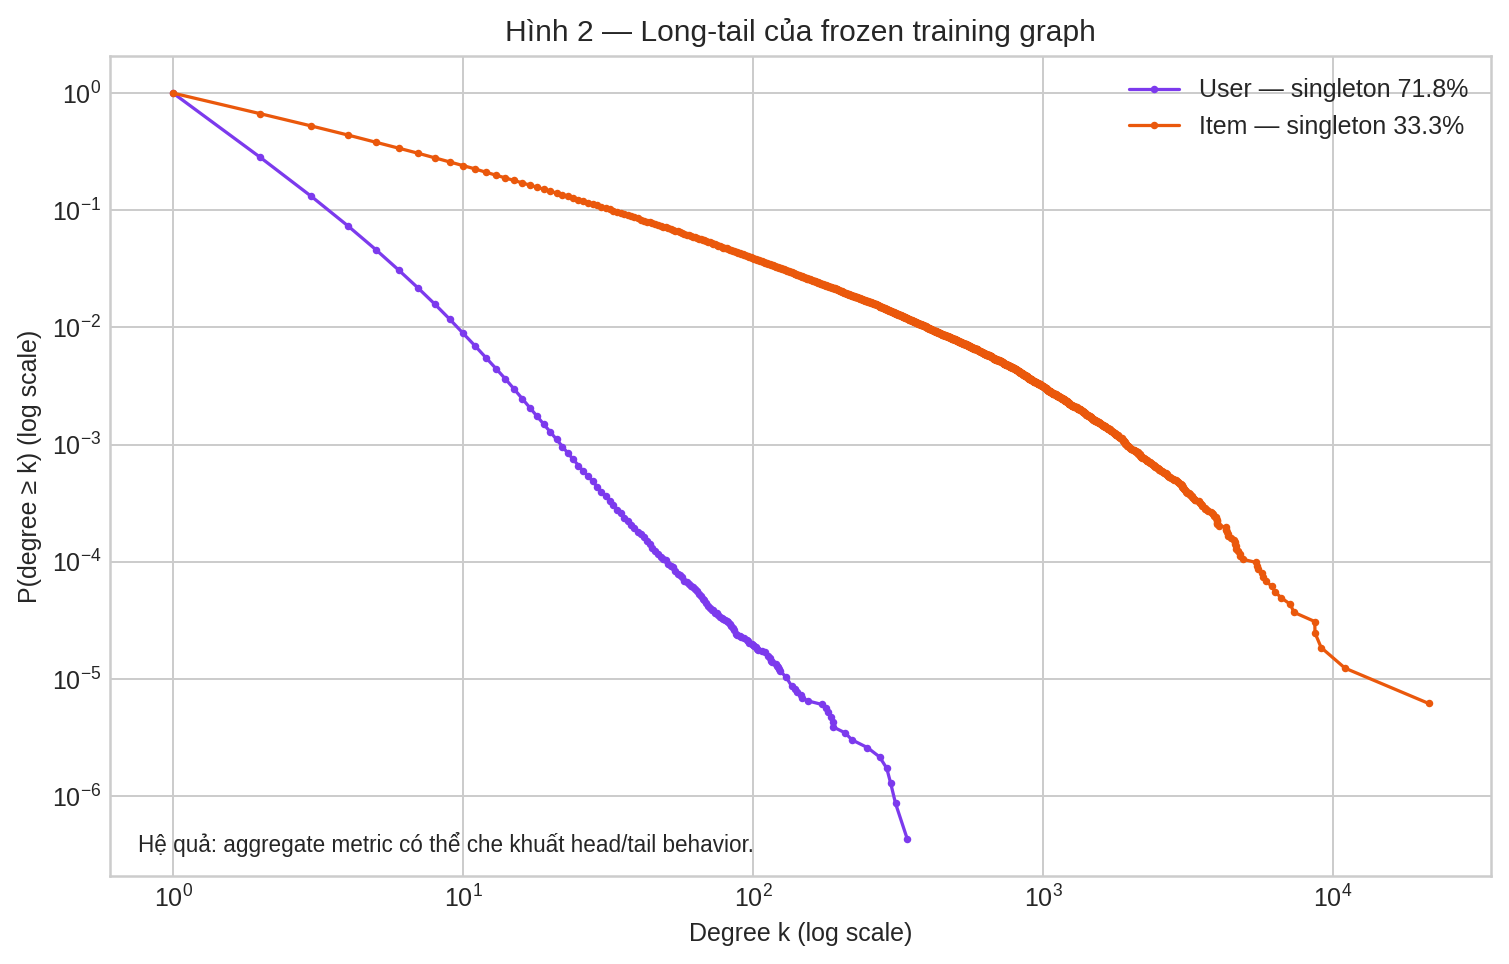
\includegraphics[width=0.49\linewidth]{02_degree_long_tail.png}\hfill
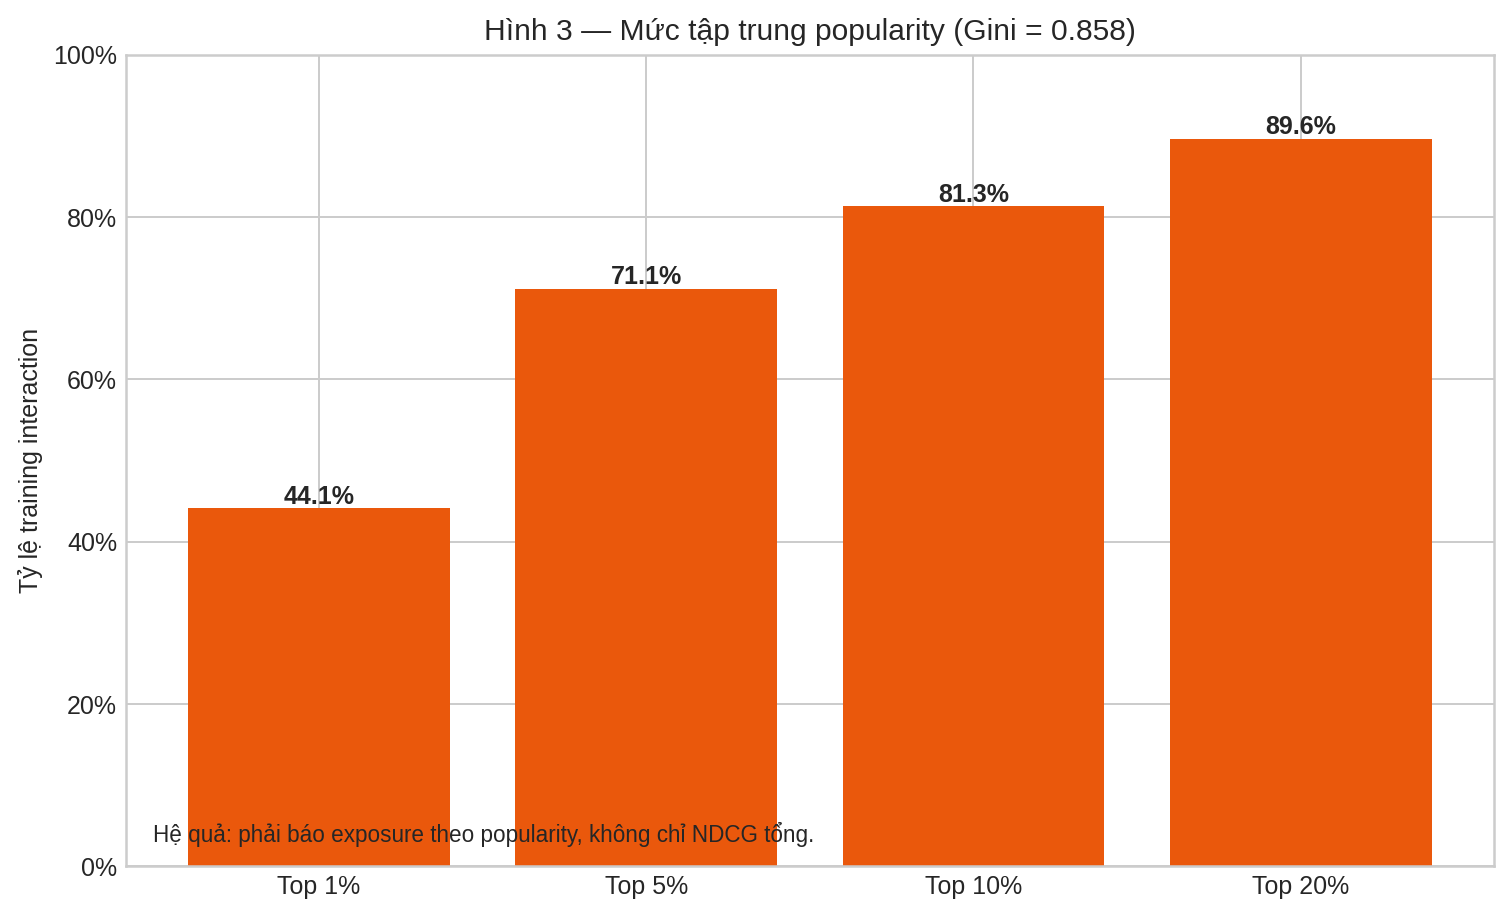
\includegraphics[width=0.49\linewidth]{03_item_concentration.png}
\caption{Trái: phân phối bậc (log--log). Phải: tỷ lệ tương tác do sản phẩm phổ biến nhất nắm giữ.}\label{fig:longtail}
\end{figure}

Gini bậc sản phẩm 0,8584; top 1\% sản phẩm giữ 44,09\% tương tác, top 20\% giữ 89,65\%. Nhóm theo bậc (khóa trước khi có kết quả model): head ($\ge$397) có 1,00\% sản phẩm và 44,16\% cạnh; body (13--396) 18,92\% và 45,45\%; tail ($\le$12) 80,07\% và 10,39\%. Hệ quả: chỉ số tổng có thể tăng chỉ nhờ phục vụ tốt sản phẩm phổ biến; mọi kết quả phải kèm exposure và hit theo nhóm.

\section{Không đủ dữ liệu: cold-start}
\begin{figure}[h]
\centering
\begin{tikzpicture}
\begin{axis}[xbar stacked, width=0.95\linewidth, height=2.6cm, bar width=16pt, xmin=0, xmax=100, ytick=\empty, xlabel={\% của 373.776 tương tác P4 trong cửa sổ validation},
  legend style={draw=none, font=\small, legend columns=2}, legend pos=outer north east, legend to name=coldleg, axis lines*=left]
\addplot[fill=teal, draw=none] coordinates {(21.90,0)};
\addplot[fill=coral, draw=none] coordinates {(64.18,0)};
\addplot[fill=coral!50, draw=none] coordinates {(9.25,0)};
\addplot[fill=amber, draw=none] coordinates {(4.67,0)};
\legend{Warm (21,9\%), User mới (64,2\%), User và sản phẩm mới (9,2\%), Sản phẩm mới (4,7\%)}
\end{axis}
\end{tikzpicture}\\[2pt]
\ref{coldleg}
\caption{Thành phần tương tác tương lai so với graph train.}\label{fig:cold}
\end{figure}

71,76\% user train chỉ có một tương tác. Trong cửa sổ validation, 73,4\% tương tác đến từ user chưa có trong train; chỉ 21,9\% dùng được cho gợi ý warm-start, và con số này giảm còn 9,8\% ở cửa sổ test. Đồ án giới hạn ở warm-start; cold-start cần feature nội dung và là hướng phát triển. Các số trên chỉ là số đếm dòng, không dùng target để thiết kế.

\section{Dữ liệu theo thời gian}
\begin{figure}[h]
\centering
\begin{tikzpicture}
\begin{axis}[ybar, width=0.95\linewidth, height=5cm, bar width=9pt, xmin=2009.5, xmax=2023.5, ymin=0,
  xtick={2010,2012,...,2022}, xticklabel style={/pgf/number format/.cd, set thousands separator={}}, ylabel={nghìn tương tác P4},
  axis lines*=left]
\addplot[fill=tealmid, draw=none] coordinates {(2010,21.2) (2011,43.1) (2012,56.7) (2013,140.7) (2014,217.2) (2015,346.7) (2016,417.4) (2017,414.2) (2018,497.6) (2019,664.8) (2020,638.0) (2021,533.7) (2022,438.3) (2023,190.7)};
\draw[dashed, coral, thick] (axis cs:2020.68,0) -- (axis cs:2020.68,700) node[above, font=\scriptsize] {$t_0$};
\draw[dashed, coral, thick] (axis cs:2021.61,0) -- (axis cs:2021.61,700) node[above, font=\scriptsize] {$t_1$};
\draw[dashed, coral, thick] (axis cs:2022.54,0) -- (axis cs:2022.54,700) node[above, font=\scriptsize] {$t_2$};
\end{axis}
\end{tikzpicture}
\caption{Tương tác 4--5\rstar{} theo năm (2023 chỉ đến tháng 9).}\label{fig:year}
\end{figure}

Dữ liệu trải từ 10/06/2000 đến 12/09/2023, tăng mạnh từ 2013, đỉnh 2019--2020 rồi giảm. Phân bố thay đổi theo thời gian nên đồ án chia theo thời gian thay vì ngẫu nhiên: $t_1$ = 11/08/2021, $t_2$ = 16/07/2022. Cửa sổ development $[t_0, t_1)$ với $t_0$ = 05/09/2020 có 553.157 tương tác P4.

\subsection*{Hành vi theo thời gian và độ trôi}
\begin{figure}[h]
\centering
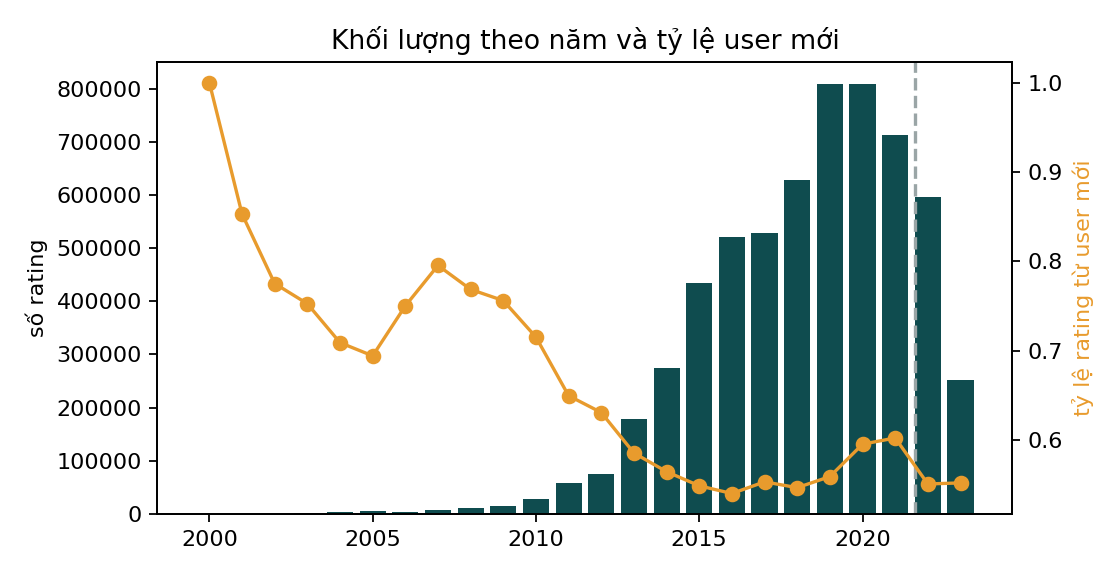
\includegraphics[width=0.49\linewidth]{D2_yearly_volume_new_users.png}\hfill
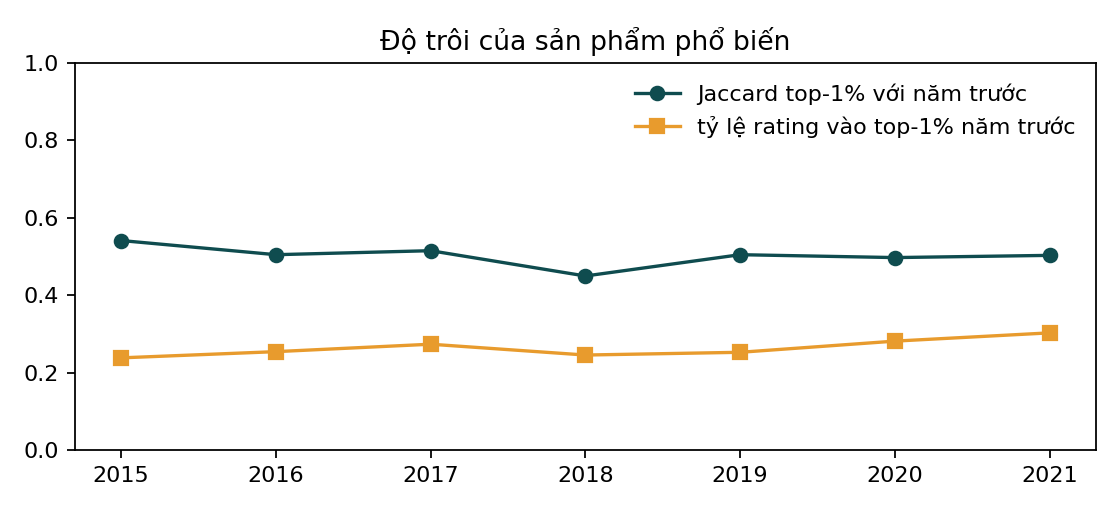
\includegraphics[width=0.49\linewidth]{D3_popularity_drift.png}
\caption{Trái: khối lượng và tỷ lệ rating từ user mới theo năm. Phải: độ trôi của top 1\% sản phẩm.}\label{fig:drift}
\end{figure}
Mỗi năm từ 2014 đến 2023, 55--60\% rating đến từ user lần đầu xuất hiện. Khoảng cách trung vị giữa hai tương tác của cùng user là 20,9 ngày (p90: 598 ngày), và 41,4\% cặp tương tác liên tiếp nằm trong cùng một ngày: user thường đánh giá theo đợt. Sản phẩm có $\ge$2 rating hoạt động trung vị 565 ngày. Top 1\% sản phẩm phổ biến của năm sau chỉ trùng khoảng một nửa với năm trước (Jaccard 0,45--0,54 giai đoạn 2015--2021); tỷ lệ rating vào top 1\% của năm trước là 24--30\%, thấp hơn 31--34\% của top 1\% chính năm đó. Rating trung bình theo năm đạt 4,35 năm 2019 rồi giảm còn 4,06 năm 2022. Hệ quả: chia theo thời gian là cần thiết, và sampler dựa trên bậc tích lũy (M1) có thể bám vào sản phẩm đã hết thời.

\subsection*{Development split (gate R1)}
Quy tắc chính được áp dụng, không cần dự phòng: $t_0$ = 05/09/2020. $G_{\text{dev\_train}}$ có 3.315.497 cạnh (85,7\% graph train hiện tại), 1.965.541 user, 144.011 sản phẩm. Cửa sổ $[t_0, t_1)$ có 553.157 tương tác P4, trong đó 105.401 target warm (19,1\%); 77,2\% bị loại vì user mới. Mọi cạnh train có timestamp nhỏ hơn mọi target, mọi dòng trước $t_1$, không dùng dòng validation/test; SHA-256 của bốn file được ghi trong \texttt{development\_graph\_manifest.json} và kiểm tra bởi \texttt{tests/test\_grapes\_gfn\_rec\_protocol.py}.

\section{Cấu trúc graph huấn luyện}
Graph train có 2.480.433 node và 3.868.654 cạnh (mật độ $1{,}03\times10^{-5}$). 96,50\% node thuộc thành phần liên thông lớn nhất (34.288 thành phần). Graph gần như liên thông nên lan truyền 2--3 bước chạm tới phần lớn graph; mỗi lựa chọn node vì vậy đánh đổi giữa tín hiệu phổ biến (dễ có, ít tính cá nhân) và tín hiệu hiếm.

\subsection*{Đồng mua và bằng chứng collaborative cho target}
Graph train có 4.887.104 cặp sản phẩm đồng mua (cùng ít nhất một user); trung vị mỗi sản phẩm có 5 sản phẩm đồng mua (p90: 106). Tuy vậy 33.560 sản phẩm (20,7\%) không có sản phẩm đồng mua nào vì chỉ được user một-tương-tác chạm tới; tỷ lệ này là 0\% ở head, 0,13\% ở body và 25,8\% ở tail. Những sản phẩm này không nhận được collaborative signal qua đường sản phẩm--user--sản phẩm; không sampler nào tạo ra tín hiệu không tồn tại.

\begin{table}[h]
\centering\small
\caption{Target development: nhóm sản phẩm và bằng chứng đồng mua (20.000 target mẫu, graph $G_{\text{dev\_train}}$).}\label{tab:reach}
\begin{tabular}{lrrrr}
\toprule
 & Head & Body & Tail & Tất cả \\
\midrule
\% sản phẩm trong catalog & 1,0 & 19,0 & 80,0 & 100 \\
\% target & 37,3 & 49,8 & 12,9 & 100 \\
\% target có đường user$\rightarrow$SP$\rightarrow$user$\rightarrow$target & 53,0 & 16,9 & 4,5 & 29,0 \\
\bottomrule
\end{tabular}
\end{table}
Chỉ 29,0\% target có đường đi độ dài 3 từ user tới target trong graph train, tức có một user khác đã mua cả sản phẩm của user lẫn target. Với tail con số là 4,5\%. Điểm số LightGCN là tích vô hướng giữa hai embedding đã lan truyền nên vẫn có thể xếp hạng target xa hơn, nhưng bằng chứng collaborative trực tiếp là rất hạn chế. 46,5\% target thuộc user chỉ có một tương tác train. Quyết định (DL-003): mọi kết quả holdout được báo thêm theo nhóm có/không có đường độ dài $\le$3.

\section{Metadata sản phẩm}
Amazon Reviews'23 công bố \texttt{meta\_Baby\_Products} với title, categories (phân cấp), features, description, price, store, details \cite{amazon23}. Metadata cho phép đo mức khớp ngữ nghĩa và đa dạng (mục~\ref{sec:semantic}) mà không thay đổi phương pháp.

\begin{figure}[h]
\centering
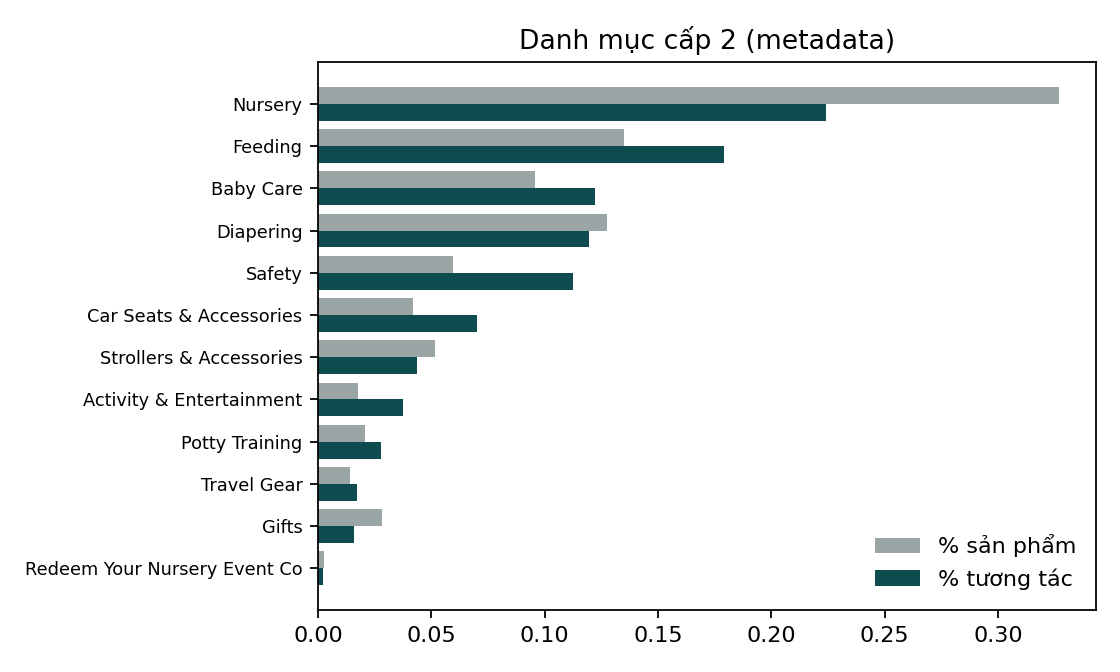
\includegraphics[width=0.62\linewidth]{D6_metadata_categories.png}
\caption{Danh mục cấp 2: tỷ lệ sản phẩm và tỷ lệ tương tác.}\label{fig:meta}
\end{figure}
Metadata phủ 100\% sản phẩm train. Độ phủ theo trường: title 99,99\%, store 98,5\%, danh mục 93,4\%, features 77,6\%, mô tả 62,3\%, giá chỉ 22,6\%. Cây danh mục chủ yếu sâu 4--5 cấp, gồm 96 danh mục cấp 2 và 448 danh mục lá; chỉ 61\% sản phẩm có \texttt{main\_category} là ``Baby'' (tiếp theo là Amazon Home 13,3\%, Health \& Personal Care 4,7\%). Phân bổ theo danh mục cũng lệch: Nursery chiếm 32,7\% sản phẩm nhưng 22,4\% tương tác, Safety 6,0\% sản phẩm nhưng 11,3\% tương tác, Feeding 13,5\% và 17,9\%. Giá trung vị gần như bằng nhau ở head (20,04), body (18,99) và tail (19,47). Kết luận: title và danh mục đủ để đo semantic match và ILD; không dùng giá.

\section{Đường đi dữ liệu và chia split}
Raw CSV (kiểm SHA-256) $\rightarrow$ kiểm toán $\rightarrow$ P4 $\rightarrow$ chia theo thời gian $\rightarrow$ graph train và mapping ID $\rightarrow$ huấn luyện có lấy mẫu $\rightarrow$ đánh giá full-graph, toàn catalog.

\begin{table}[h]
\centering\small
\caption{Vai trò các split.}\label{tab:splits}
\begin{tabularx}{\linewidth}{lYY}
\toprule
Split & Dùng cho & Cấm \\
\midrule
$G_{\text{dev\_train}}$ ($<t_0$) / $D_{\text{dev}}$ ($[t_0,t_1)$) & Chọn budget, $\alpha$, learning rate, kiến trúc; kiểm tra backbone & Kết luận cuối \\
Graph train ($<t_1$) / validation & So sánh ghép cặp sau freeze & Mọi điều chỉnh \\
Test ($\ge t_2$) & Một lần, nếu có protocol riêng & Chọn phương pháp \\
\bottomrule
\end{tabularx}
\end{table}
Quy tắc dự phòng: nếu $D_{\text{dev}}$ dưới 20.000 target hoặc $G_{\text{dev\_train}}$ mất quá 50\% cạnh, chọn $t_0$ sao cho $G_{\text{dev\_train}}$ giữ 80\% cạnh.

\section{Từ dữ liệu đến quyết định thiết kế}
\begin{table}[h]
\centering\small
\begin{tabularx}{\linewidth}{YY}
\toprule
Quan sát & Quyết định \\
\midrule
Rating hình chữ J, 21,8\% là 1--3\rstar{} & Positive = 4--5\rstar{}; không dùng rating làm trọng số \\
Nhiễu dạng lỗi 1 dòng; bất thường $<$1\% tương tác & Không lọc thêm; ghi nhận hạn chế \\
71,8\% user và 33\% sản phẩm có 1 tương tác & Không lọc $k$-core; theo dõi bậc của node được sampler chọn \\
Top 1\% sản phẩm giữ 44\% tương tác & Báo exposure/hit theo head--body--tail \\
73\% tương tác validation của user mới & Giới hạn warm-start \\
Phân bố thay đổi mạnh theo năm & Chia theo thời gian; development split trước $t_1$ \\
Graph gần liên thông, bậc kỳ vọng theo cạnh ~1.009 & Lấy mẫu có budget $k$; tính chi phí sampler \\
Batch 65.536 triplet chạm 87\% graph ngay bước 1 & Budget R3 bắt đầu từ batch $\le$4.096 cho mọi sampler \\
Chỉ 29\% target có đường độ dài 3; tail 4,5\% & Báo kết quả theo nhóm có/không có đường $\le$3 (DL-003) \\
Top 1\% sản phẩm đổi khoảng một nửa mỗi năm & Theo dõi M1 bám sản phẩm cũ \\
Metadata: title $\approx$100\%, danh mục 93\%, giá 23\% & Đo ngữ nghĩa bằng title và danh mục, không dùng giá \\
\bottomrule
\end{tabularx}
\end{table}

%=====================================================================
\chapter{Trả lời góp ý của giảng viên (3/9)}\label{ch:feedback}
Mỗi mục trình bày: câu hỏi, phân tích, số liệu và hệ quả cho thiết kế.

\section{``Converat'' — coverage và conversion}
\textbf{Coverage@20} là tỷ lệ sản phẩm trong catalog xuất hiện ít nhất một lần trong top-20 của mọi user; đo độ phủ, chưa đo ý nghĩa. \textbf{Conversion} là tỷ lệ gợi ý dẫn tới mua; cần log hiển thị--click--mua và A/B test online, dữ liệu review offline không có. Proxy offline gần nhất là Recall@20 trên tương tác tương lai. Ví dụ baseline sanity cũ: MostPop chỉ gợi ý 25 sản phẩm (coverage 0,00015) trong khi BPR-MF đạt 0,0335.

\section{Context}
Trong đồ án, \emph{context} là tập node và cạnh lân cận model dùng để tính embedding cho batch ở mỗi layer ($K^l$). Sampler quyết định context. Đây không phải ngữ cảnh người dùng như thời gian, thiết bị, vị trí (context-aware recommendation, ngoài phạm vi).

\section{NDCG}
Mỗi dòng đánh giá có một sản phẩm đúng. Xếp hạng toàn bộ catalog hợp lệ, gọi $r$ là hạng của sản phẩm đúng \cite{ndcg}:
\[
\mathrm{NDCG@20} = \begin{cases} 1/\log_2(r+1) & r \le 20 \\ 0 & r > 20 \end{cases}
\]
Hạng 1 cho 1; hạng 3 cho 0,5; hạng 10 cho 0,289; hạng 20 cho 0,228. NDCG thưởng việc đặt sản phẩm đúng lên cao; Recall@20 chỉ hỏi có vào top-20 hay không.

\section{Mức khớp ngữ nghĩa và đa dạng sản phẩm được gợi ý}\label{sec:semantic}
Với metadata, đồ án đề xuất ba phép đo bổ sung (cần giảng viên duyệt, OD-2), tính trên rank vector đã lưu nên không thay đổi phương pháp:
\begin{itemize}
\item \textbf{Semantic match@20}: $\max_{j\in\text{top-20}} \cos(e_j, e_{\text{đúng}})$, với $e$ là embedding văn bản title + features \cite{sbert}.
\item \textbf{ILD@20} \cite{ziegler}: $\frac{2}{k(k-1)}\sum_{i<j} d(i,j)$, với $d$ là $1-$Jaccard của đường danh mục hoặc $1-\cos$ văn bản.
\item \textbf{Đa dạng toàn hệ thống}: Coverage@20, Gini exposure, số danh mục xuất hiện trong gợi ý.
\end{itemize}

Metadata đủ cho các phép đo này: title 99,99\% và danh mục 93,4\% sản phẩm train (mục 2.10).

\pending{R5}{Giá trị semantic match@20 và ILD@20 cho từng phương pháp.}

\section{Tính phân bổ}
Exposure theo nhóm = tỷ lệ vị trí trong top-20 thuộc head/body/tail; hit theo nhóm = tỷ lệ target của nhóm được gợi ý đúng; Gini exposure đo mức dồn. Exposure tail tăng không đồng nghĩa hit tail tăng, nên báo cả hai.

\section{Trade-off và ``quan tâm tiêu chí nào thì giá trị khác ra sao''}
\begin{table}[h]
\centering\small
\caption{Nếu chỉ tối ưu một tiêu chí.}\label{tab:tradeoff}
\begin{tabularx}{\linewidth}{p{2.3cm}YYp{2.8cm}}
\toprule
Tối ưu & Thường xảy ra & Bằng chứng trên Baby & Cách đo \\
\midrule
NDCG tổng & Dồn về sản phẩm phổ biến & MostPop: NDCG@20 0,0059, 25 sản phẩm, 100\% exposure head & NDCG + coverage + exposure \\
Độ phủ/đa dạng & Có thể giảm độ chính xác & BPR-MF: coverage 0,0335 ($\approx$218$\times$ MostPop), NDCG@20 0,0041 & NDCG--coverage \\
Chi phí thấp (budget nhỏ) & Ít ngữ cảnh & Chưa đo (RQ4) & NDCG--thời gian \\
Đưa tail lên & Exposure tăng, hit chưa chắc & Chưa đo & Exposure và hit tail \\
Khớp ngữ nghĩa & Gợi ý giống nhau & Chưa đo & Semantic match + ILD \\
\bottomrule
\end{tabularx}
\end{table}
MostPop, BPR-MF là baseline sanity cũ (5 epoch, validation), chỉ minh họa trade-off. Kết quả cuối được trình bày như mặt trận Pareto: một phương pháp không được coi là tốt hơn nếu thua ở một trục mà không thắng ở trục khác.

\section{Phân tích dữ liệu ban đầu}
Các câu hỏi về số sản phẩm, histogram, mất cân bằng, dồn về, không đủ dữ liệu, rating, cách biểu diễn, nhiễu và cân bằng được trả lời trong chương~\ref{ch:data}: mục 2.1--2.9 và Bảng~\ref{tab:noise}, \ref{tab:policy}.

\section{Sampling hay distributed}
Xem mục~\ref{sec:dist}: chọn sampling; distributed bổ sung, không thay thế.

\section{Long-tail và quan hệ giữa các node có giá trị ra sao}
\begin{itemize}
\item \textbf{user$\rightarrow$sản phẩm}: lịch sử trực tiếp; với user một tương tác đây là toàn bộ thông tin.
\item \textbf{sản phẩm$\rightarrow$user$\rightarrow$sản phẩm}: ``người mua A cũng mua B'', collaborative signal cốt lõi, xuất hiện từ bước 2.
\item \textbf{qua sản phẩm head}: nhiều tín hiệu phổ biến, ít tính cá nhân, tốn chi phí lan truyền.
\item \textbf{qua sản phẩm tail}: tín hiệu riêng, ngách, ít quan sát nên dễ nhiễu.
\item \textbf{qua user hoạt động nhiều}: cầu nối nhiều sản phẩm, có thể quá chung.
\end{itemize}
Heuristic cố định áp đặt trước giá trị (M1 ưu tiên head, M2 phạt hub). GRAPES-GFN-Rec để sampler học: quan hệ nào giúp BPR loss giảm sẽ được chọn nhiều hơn; RQ3 đo lại phân phối node được chọn và RQ4 cho biết quan hệ nào vẫn được giữ khi budget chặt.

Số liệu đã có (mục 2.9): 20,7\% sản phẩm (25,8\% tail) không có sản phẩm đồng mua; chỉ 29,0\% target development có đường độ dài 3 từ user (head 53,0\%, body 16,9\%, tail 4,5\%). Quan hệ qua head vì vậy mang phần lớn bằng chứng collaborative, còn tail gần như không có — đây chính là chỗ một sampler học được có thể hoặc khuếch đại thiên lệch, hoặc tìm được đường gián tiếp có ích.

\pending{R6}{Phân phối node được sampler chọn theo layer, so với M0/M1.}

\chapter{Phương pháp GRAPES-GFN-Rec}

\section{Kiến trúc tổng thể}
\begin{figure}[h]
\centering
\begin{tikzpicture}[
  node distance=0.5cm and 0.35cm,
  b/.style={draw=none,rounded corners=3pt,fill=tealpale,align=center,font=\sffamily\small,minimum height=1.0cm,text width=2.2cm},
  d/.style={b,fill=teal,text=white},
  o/.style={b,fill=amberpale},
  a/.style={b,fill=amber},
  ar/.style={-{Stealth[length=2.5mm]},thick,gray}]
\node[b] (batch) {Batch BPR\\$(u,i^+,i^-)$};
\node[b,right=of batch] (v0) {$V^0$ = tập\\endpoint};
\node[d,right=of v0,text width=3.6cm] (s) {Sampler $\mathrm{GCN}_S$\\\mbox{Gumbel Top-$k$}\\mỗi layer};
\node[d,right=of s,text width=3.3cm] (r) {Sampled LightGCN\\trên $K^1,\dots,K^L$};
\node[o,below=of r,text width=3.3cm] (bpr) {BPR loss\\$\rightarrow$ cập nhật $\Theta_R$};
\node[b,below=of s,text width=3.6cm] (lq) {$\log q = \sum_l \log q_l$};
\node[b,below=of v0,text width=2.4cm] (lz) {$\mathrm{GCN}_Z$\\$\rightarrow \log Z(V^0)$};
\node[a,below=0.6cm of lq,text width=12.2cm] (tb) {Trajectory Balance: $\big(\log Z + \log q + \alpha\cdot\mathrm{sg}(L_{\text{BPR}})\big)^2 \rightarrow$ cập nhật $\Theta_S \cup \Theta_Z$};
\draw[ar] (batch)--(v0); \draw[ar] (v0)--(s); \draw[ar] (s)--(r);
\draw[ar] (r)--(bpr); \draw[ar] (s)--(lq); \draw[ar] (v0)--(lz);
\draw[ar] (lz.south) -- (lz.south |- tb.north);
\draw[ar] (lq)--(tb);
\draw[ar] (bpr.south) -- (bpr.south |- tb.north);
\end{tikzpicture}
\caption{Một bước huấn luyện. $\mathrm{sg}$ là stop-gradient. Suy luận không lấy mẫu: LightGCN chạy trên toàn graph train, xếp hạng toàn catalog.}\label{fig:arch}
\end{figure}

Hình~\ref{fig:arch} là khung kiến trúc chung. Sampler và recommender có tham số, optimizer và gradient tách biệt. Backbone có thể thay (ví dụ NGCF, SGL) mà không đổi sampler; trong triển khai thực tế, sampler chỉ dùng lúc huấn luyện, phục vụ gợi ý dùng embedding đã học.

\section{Chuyển đổi từ GRAPES sang gợi ý}
\begin{table}[h]
\centering\small
\caption{Chuyển đổi thành phần. Các dòng bên phải là quyết định thiết kế của đồ án, không phải kết quả đã được paper GRAPES chứng minh.}\label{tab:adapt}
\begin{tabularx}{\linewidth}{lYY}
\toprule
Khía cạnh & GRAPES gốc & GRAPES-GFN-Rec \\
\midrule
Đồ thị & Node có feature & Hai phía user--item, chỉ positive trước mốc thời gian \\
Mục tiêu batch & Node có nhãn & Triplet BPR; $V^0$ = unique endpoint, giữ ánh xạ triplet \\
Feature sampler & Feature node & Embedding ID riêng, one-hot loại node, $\log(1+\deg)$ chuẩn hóa, cờ lịch sử $L{+}1$ kênh \\
Model chính & GCN phân loại & Sampled LightGCN: không self-loop, block $K^l \rightarrow K^{l-1}$, bi-normalization chữ nhật \\
Chi phí & Cross-entropy & Mean BPR loss, không gồm regularizer \\
$\log Z$ & GCN trên target và hàng xóm & $\mathrm{GCN}_Z$ chỉ trên $V^0$ \\
Đánh giá & Accuracy & Xếp hạng toàn catalog, NDCG@20, Recall@20, coverage, head/tail \\
\bottomrule
\end{tabularx}
\end{table}

\section{Lấy mẫu theo layer}
Với mỗi layer $l = 1,\dots,L$, tập ứng viên là hàng xóm của trạng thái trước trừ chính nó:
\[
C^l = \mathcal{N}_{G_{\text{train}}}(K^{l-1}) \setminus K^{l-1}, \qquad K^0 = V^0.
\]
$\mathrm{GCN}_S$ hai lớp chạy trên subgraph cảm sinh bởi $K^{l-1}\cup C^l$ và cho logit $\ell_v$, xác suất $p_v = \sigma(\ell_v)$ cho mỗi $v\in C^l$. Hành động chọn đúng $\min(k_l,|C^l|)$ node:
\[
V^l = \operatorname{TopK}_{v\in C^l}\big(\log p_v + g_v\big),\quad g_v\sim\mathrm{Gumbel}(0,1), \qquad K^l = V^0 \cup V^l.
\]
Log-likelihood dùng phân phối Bernoulli đầy đủ, gồm cả node được chọn ($m_v=1$) và không được chọn:
\[
\log q_l = \sum_{v\in C^l} \big[m_v \log p_v + (1-m_v)\log(1-p_v)\big], \qquad \log q = \sum_{l=1}^{L} \log q_l.
\]
Hành động lấy từ phân phối exact-$k$ trong khi likelihood là Bernoulli không điều kiện: đây là sai lệch off-policy kế thừa từ GRAPES và sẽ được nêu rõ.

Hai đối chứng M0 và M1 dùng cùng đường code, chỉ khác điểm: M0 dùng điểm bằng nhau, M1 dùng $\log\deg(v)$; cả hai không có tham số và $\log q = 0$. Nhờ vậy khác biệt giữa các sampler chỉ nằm ở cách chấm điểm.

\section{Sampled LightGCN}
Block $P_l \in \mathbb{R}^{|K^{l-1}|\times|K^l|}$ chứa cạnh gốc giữa nguồn $K^l$ và đích $K^{l-1}$, chuẩn hóa hai phía theo bậc cục bộ trong block:
\[
P_l[t,s] = \frac{B_l[t,s]}{\sqrt{d^{\text{dst}}_l(t)\, d^{\text{src}}_l(s)}}.
\]
Embedding ở độ sâu $r$ của $V^0$ là tích tiền tố $e^{r} = P_1 P_2\cdots P_r\, E[K^r]$, và biểu diễn cuối là trung bình đều $z = \frac{1}{L+1}\sum_{r=0}^{L} e^{r}$.

\paragraph{Giới hạn đã được chứng minh bằng test.} Vì $K^l$ không cộng dồn, khi $V^0$ chứa cả user lẫn item, một số node thuộc $V^1$ bị loại khỏi $K^2$; do đó kể cả khi lấy hết ứng viên, kết quả không bằng Full LightGCN. Với target chỉ gồm một user, hai cách cho kết quả bằng nhau. Đây là tính chất của cách định nghĩa trạng thái trong GRAPES, không phải lỗi cài đặt.

\section{Hàm mục tiêu}
Recommender tối ưu
\[
L_{\text{BPR}} = -\frac{1}{M}\sum_{b=1}^{M}\log\sigma\big(z_{u_b}^\top z_{i_b^+} - z_{u_b}^\top z_{i_b^-}\big), \qquad L_{\text{model}} = L_{\text{BPR}} + \lambda\,L_{\text{reg}}.
\]
Sampler tối ưu Trajectory Balance \cite{tb} với phần thưởng $R = \exp(-\alpha L_{\text{BPR}})$:
\[
L_{\text{TB}} = \Big(\log Z(V^0) + \log q + \alpha\cdot\mathrm{sg}(L_{\text{BPR}})\Big)^2.
\]
$\log Z(V^0)$ là trung bình đầu ra của $\mathrm{GCN}_Z$ trên subgraph cảm sinh bởi $V^0$ (có self-loop), nên bất biến với hoán vị và với node ngoài $V^0$. Biến thể GRAPES-RL-Rec thay $L_{\text{TB}}$ bằng $\mathrm{sg}(L_{\text{BPR}})\cdot\log q$.

\begin{algorithm}[h]
\small
\caption{Một bước huấn luyện GRAPES-GFN-Rec}
\KwIn{batch triplet $B$, graph $G_{\text{train}}$, budget $(k_1,\dots,k_L)$, $\alpha$}
$V^0 \leftarrow \mathrm{unique}(B)$; giữ ánh xạ triplet $\rightarrow$ chỉ số\;
\For{$l \leftarrow 1$ \KwTo $L$}{
  $C^l \leftarrow \mathcal{N}(K^{l-1})\setminus K^{l-1}$;\quad $\ell \leftarrow \mathrm{GCN}_S(K^{l-1}\cup C^l)$\;
  $V^l \leftarrow \mathrm{GumbelTopK}(\log\sigma(\ell), k_l)$;\quad $\log q \mathrel{+}= \log q_l$;\quad $K^l \leftarrow V^0\cup V^l$\;
}
$z \leftarrow \mathrm{SampledLightGCN}(P_1,\dots,P_L)$;\quad tính $L_{\text{model}}$\;
Cập nhật $\Theta_R$ bằng $\nabla L_{\text{model}}$ \tcp*{sampler không nhận gradient này}
$L_{\text{TB}} \leftarrow (\log Z(V^0) + \log q + \alpha\,\mathrm{sg}(L_{\text{BPR}}))^2$\;
Cập nhật $\Theta_S\cup\Theta_Z$ bằng $\nabla L_{\text{TB}}$ \tcp*{recommender không nhận gradient này}
Ghi log: $L_{\text{BPR}}$, $L_{\text{TB}}$, $\log q$, $\log Z$, $|C^l|$, $|V^l|$, bậc/loại/nhóm của $V^l$, thời gian, bộ nhớ\;
\end{algorithm}

\section{Những điểm riêng của bài toán gợi ý}
\begin{description}[style=nextline,leftmargin=1.2cm]
\item[R-1 Quá ít phần thưởng.] Pilot dùng batch 65.536 trong 5 epoch, khoảng 300 bước tối ưu: sampler chỉ nhận khoảng 300 phần thưởng vô hướng cho hàng trăm nghìn node mục tiêu mỗi bước. GRAPES gốc dùng batch 256--512. Batch và budget sẽ được chọn lại trên development split, chung cho mọi sampler.
\item[R-2 Thang phần thưởng.] BPR khởi đầu khoảng 0,69 và chênh lệch giữa trajectory rất nhỏ; nếu $\alpha$ quá nhỏ, $\log q$ lấn át phần thưởng. GRAPES gốc chọn hệ số trong khoảng $10^3$ đến $10^5$. $\alpha$ và $\log Z$ khởi đầu được quét trên $D_{\text{dev}}$.
\item[R-3 Phần thưởng không dừng.] Khi recommender học thêm, cùng trajectory cho loss khác. Giữ như GRAPES và ghi log mức trôi.
\item[R-4 Graph cực thưa.] Theo dõi phân phối bậc, loại và nhóm của node được chọn để phát hiện sampler dồn về hub.
\item[R-5 Chi phí sampler.] Embedding cho 2,48 triệu node cộng $\mathrm{GCN}_S$ có thể đắt hơn LightGCN; chi phí báo cáo gồm cả sampler.
\item[R-6 Backbone yếu.] Trong pilot, Full LightGCN (NDCG@20 0,0049) thua MostPop (0,0059). Full LightGCN phải vượt MostPop trên $D_{\text{dev}}$ trước khi so sánh sampler có ý nghĩa.
\item[R-7, R-8.] Item âm cũng là mục tiêu của sampler; cạnh positive của batch có thể rò qua propagation, được kiểm tra bằng ablation che cạnh tạm thời.
\end{description}

\chapter{Thiết kế thực nghiệm}

\section{Phương pháp so sánh}
\begin{table}[h]
\centering\small
\caption{Các phương pháp so sánh.}\label{tab:comp}
\begin{tabularx}{\linewidth}{llYY}
\toprule
Tầng & Phương pháp & Vai trò & Câu hỏi trả lời \\
\midrule
A & GRAPES-GFN-Rec & Phương pháp đề xuất & -- \\
A & M0 Uniform & Đối chứng trung lập & Học có hơn chọn ngẫu nhiên? \\
A & M1 Degree-importance & Đối chứng tĩnh (họ FastGCN/LADIES \cite{fastgcn,ladies}) & Học có hơn ưu tiên node phổ biến? \\
A & GRAPES-RL-Rec & Ablation hàm mục tiêu & TB có cần hơn REINFORCE? \\
B & Full LightGCN & Không lấy mẫu & Lấy mẫu mất bao nhiêu chất lượng? \\
B & MostPop, BPR-MF & Sanity & Graph có giá trị? \\
C & GraphSAGE fan-out \cite{graphsage} & Tùy chọn & Layer-wise học được vs node-wise? \\
\bottomrule
\end{tabularx}
\end{table}
Tầng A dùng chung graph, thứ tự triplet, negative, khởi tạo, budget, seed, evaluator và GPU, và được chạy lại hoàn toàn; số liệu pilot không được dùng lại.

\section{Chỉ số}
\begin{itemize}
\item \textbf{Chất lượng:} NDCG@20 (chính), Recall@20; chênh lệch ghép cặp theo seed.
\item \textbf{Phân bổ và đa dạng:} Catalog Coverage@20; exposure và hit theo head/body/tail; Gini exposure.
\item \textbf{Chi phí:} thời gian sampler, TB, propagation và epoch; peak GPU memory; số node/cạnh thực tế mỗi layer.
\item \textbf{Hành vi sampler:} bậc, loại, nhóm của node được chọn; entropy; $p_{\min}, p_{\max}$; độ thay đổi tham số sampler.
\item \textbf{Ngữ nghĩa và đa dạng:} semantic match@20, ILD@20 (mục~\ref{sec:semantic}), nếu OD-2 được duyệt. Conversion không đo được offline.
\end{itemize}

\section{Tiêu chí kết luận}
Chỉ kết luận GRAPES-GFN-Rec cải thiện trade-off khi chênh lệch NDCG@20 so với đối chứng tầng A tốt nhất dương ở mọi seed holdout và chi phí được báo đầy đủ. Một run không hợp lệ nếu vi phạm cách ly thời gian, exact-$k$, quy tắc ứng viên, hướng block và normalization, tính hữu hạn của loss, phân quyền gradient, khả năng lặp lại hoặc thiếu log tài nguyên. Không đổi phương pháp, $\alpha$, budget hay seed sau khi đọc holdout.


%=====================================================================
\chapter{Kết quả}\label{ch:results}

\section{Tiến độ đã kiểm chứng}
\begin{itemize}
\item \textbf{R0}: spec chuẩn, decision log DL-001, checklist G1--G7, công cụ kiểm tra tính nhất quán.
\item \textbf{R2 (lõi)}: sampler (learned, uniform, degree), Sampled LightGCN, bước huấn luyện TB/REINFORCE. 28 oracle test pass trên PyTorch CPU: tập ứng viên khớp brute-force; exact-$k$; lấy mẫu đều khi điểm bằng nhau; $\log q$ khớp tính tay; đường đi mẫu cho 1 (không chuẩn hóa), $1/2$ (bậc toàn graph), $1/\sqrt{2}$ (bậc cục bộ); TB khớp tính tay; $\log Z$ bất biến hoán vị; TB không tạo gradient cho recommender và ngược lại; tham số sampler thay đổi sau một bước; lặp lại xác định. Bốn lỗi cài cố ý đều bị phát hiện.
\end{itemize}

\section{Development (R3)}
\pending{Notebook 12, dự kiến 23/09--10/10}{Full LightGCN vs MostPop theo số epoch; budget chung (batch, $k$, số bước, thời gian, bộ nhớ); quét $\alpha$, $\log Z$ khởi đầu, learning rate; bằng chứng sampler học (G7); chi phí sampler.}

\section{So sánh ghép cặp trên holdout (R5)}
\pending{Notebook 13, dự kiến 14/10--27/10}{NDCG@20, Recall@20 của 7 phương pháp $\times$ 3 seed và chênh lệch ghép cặp (RQ1); coverage, exposure/hit theo nhóm, Gini; thời gian và bộ nhớ; TB vs REINFORCE (RQ2); semantic match@20, ILD@20.}

\section{Hành vi sampler và độ nhạy budget (R6)}
\pending{Dự kiến 28/10--03/11}{Bậc, loại, nhóm của node được chọn theo layer so với M0/M1 (RQ3); mặt trận Pareto; budget chặt (RQ4); ablation che cạnh positive (D9) và $\log Z$ kiểu cũ (D6).}

%=====================================================================
\chapter{Kết luận và hướng phát triển}
\pending{R7, dự kiến 04/11--17/11}{Trả lời RQ1--RQ4 từ bằng chứng holdout; hạn chế (warm-start, một dataset, off-policy mismatch, $K^l$ không cộng dồn); hướng phát triển: cold-start với metadata, Home\_and\_Kitchen, distributed + sampler học được.}

\noindent\textbf{Hạn chế đã biết từ thiết kế:} chỉ warm-start; một dataset chính; sai lệch off-policy giữa hành động exact-$k$ và likelihood Bernoulli (kế thừa GRAPES); trạng thái $K^l = V^0\cup V^l$ không tương đương Full LightGCN khi $V^0$ có cả user lẫn sản phẩm; chỉ đo huấn luyện có lấy mẫu, không đo suy luận có lấy mẫu.

%=====================================================================
\appendix
\chapter{Kế hoạch đến hạn nộp 30/11/2026}
\begin{table}[h]
\centering\small
\begin{tabularx}{\linewidth}{llYl}
\toprule
Tuần & Gate & Việc & Trạng thái \\
\midrule
16/9 & R0, R2 lõi & Scope, spec, code, oracle test & Xong \\
16/9 & R1 & Notebook 11: phân tích sâu + development split & Xong \\
16--22/9 & R2 & Hoàn tất R2 (negative, D9, D6, embedding thưa) & Đang làm \\
23/9--10/10 & R3 & Backbone, budget, quét $\alpha$/lr, khả thi T4 & \\
10--13/10 & R4 & Gặp giảng viên chốt OD-1…OD-4; freeze & \\
14--27/10 & R5 & 7 phương pháp $\times$ 3 seed, chạy Colab song song & \\
28/10--3/11 & R6 & Phân tích RQ1--RQ4, ngữ nghĩa, Pareto & \\
4--17/11 & R7 & Hoàn thiện luận văn và slide (viết song song từ tuần đầu) & \\
18--30/11 & Dự phòng & Sửa theo góp ý, nộp & \\
\bottomrule
\end{tabularx}
\end{table}

\noindent\textbf{Quyết định cần giảng viên:} OD-1 thêm GraphSAGE fan-out (mặc định không); OD-2 nối metadata để đo ngữ nghĩa và đa dạng (khuyến nghị có); OD-3 lưới budget (một chính, một chặt); OD-4 số seed (3).

\chapter{Pilot M0--M2 (lưu trữ)}
Pilot so sánh ba luật chọn node cố định trên validation với batch 65.536, 5 epoch ($\approx$300 bước). Trung bình ba seed NDCG@20: M0 0,005706; M1 0,005866; M2 0,005721. M2 là heuristic tĩnh, không phải biến thể GRAPES; kết quả không dùng để chọn cấu hình hay kết luận về GRAPES-GFN-Rec. Bài học: quá ít bước cho sampler học (R-1) và backbone còn yếu (Full LightGCN 0,004931 < MostPop 0,005873, R-6).

\begin{thebibliography}{99}\small
\bibitem{grapes} T.~Younesian et al. \emph{GRAPES: Learning to Sample Graphs for Scalable Graph Neural Networks}. arXiv:2310.03399v3. Mã nguồn: \url{https://github.com/dfdazac/grapes}, commit \texttt{71ecebe}.
\bibitem{lightgcn} X.~He et al. \emph{LightGCN: Simplifying and Powering Graph Convolution Network for Recommendation}. SIGIR 2020. arXiv:2002.02126.
\bibitem{tb} N.~Malkin et al. \emph{Trajectory Balance: Improved Credit Assignment in GFlowNets}. NeurIPS 2022. arXiv:2201.13259.
\bibitem{bpr} S.~Rendle et al. \emph{BPR: Bayesian Personalized Ranking from Implicit Feedback}. UAI 2009. arXiv:1205.2618.
\bibitem{gumbeltopk} W.~Kool et al. \emph{Stochastic Beams and Where to Find Them: The Gumbel-Top-k Trick for Sampling Sequences Without Replacement}. ICML 2019. arXiv:1903.06059.
\bibitem{fastgcn} J.~Chen et al. \emph{FastGCN: Fast Learning with Graph Convolutional Networks via Importance Sampling}. ICLR 2018. arXiv:1801.10247.
\bibitem{ladies} D.~Zou et al. \emph{Layer-Dependent Importance Sampling for Training Deep and Large Graph Convolutional Networks}. NeurIPS 2019. arXiv:1911.07323.
\bibitem{graphsage} W.~Hamilton et al. \emph{Inductive Representation Learning on Large Graphs}. NeurIPS 2017. arXiv:1706.02216.
\bibitem{pinsage} R.~Ying et al. \emph{Graph Convolutional Neural Networks for Web-Scale Recommender Systems}. KDD 2018. arXiv:1806.01973.
\bibitem{amazon23} Y.~Hou et al. \emph{Bridging Language and Items for Retrieval and Recommendation}. arXiv:2403.03952. Dữ liệu: \url{https://amazon-reviews-2023.github.io/}.
\bibitem{clustergcn} W.-L.~Chiang et al. \emph{Cluster-GCN: An Efficient Algorithm for Training Deep and Large Graph Convolutional Networks}. KDD 2019. arXiv:1905.07953.
\bibitem{gas} M.~Fey et al. \emph{GNNAutoScale: Scalable and Expressive Graph Neural Networks via Historical Embeddings}. ICML 2021. arXiv:2106.05609.
\bibitem{ziegler} C.-N.~Ziegler et al. \emph{Improving Recommendation Lists Through Topic Diversification}. WWW 2005.
\bibitem{ndcg} K.~Järvelin, J.~Kekäläinen. \emph{Cumulated Gain-Based Evaluation of IR Techniques}. ACM TOIS 20(4), 2002.
\bibitem{sbert} N.~Reimers, I.~Gurevych. \emph{Sentence-BERT: Sentence Embeddings using Siamese BERT-Networks}. EMNLP 2019. arXiv:1908.10084.
\end{thebibliography}

\end{document}
